
 
HammerDB is an open source and widely used benchmark framework for the worlds most popular \gls{dbms}~\cite{scalzo2018database,elgrablyanalise,knoche2016combining,benchmarkchen,ali2019persistent,yu2015design,koccak2018software,koccak2018software}.   HammerDB emulates a \gls{tpcc} scenario  and through \gls{oltp} workloads it sets up a company's sales processing environment. It reduces the testing costs by simplifying the \gls{tpcc} rules, which can be modified and run on a custom environment. The above factors result in a low-cost solution, rapid deployment, and customized \gls{dbms} benchmark system~\cite{benchmarkchen,elgrablyanalise,hammerdb}. HammerDB currently supports Oracle, SQL Server, Db2, TimesTen, MySQL, MariaDB, PostgreSQL, Greenplum, Postgres Plus Advanced Server, and Redis. Moreover, it can run on a variety of \gls{os}, making it a  flexible and heterogeneous benchmarking framework~\cite{benchmarkchen}.


\begin{figure}[h!]
    \centering
    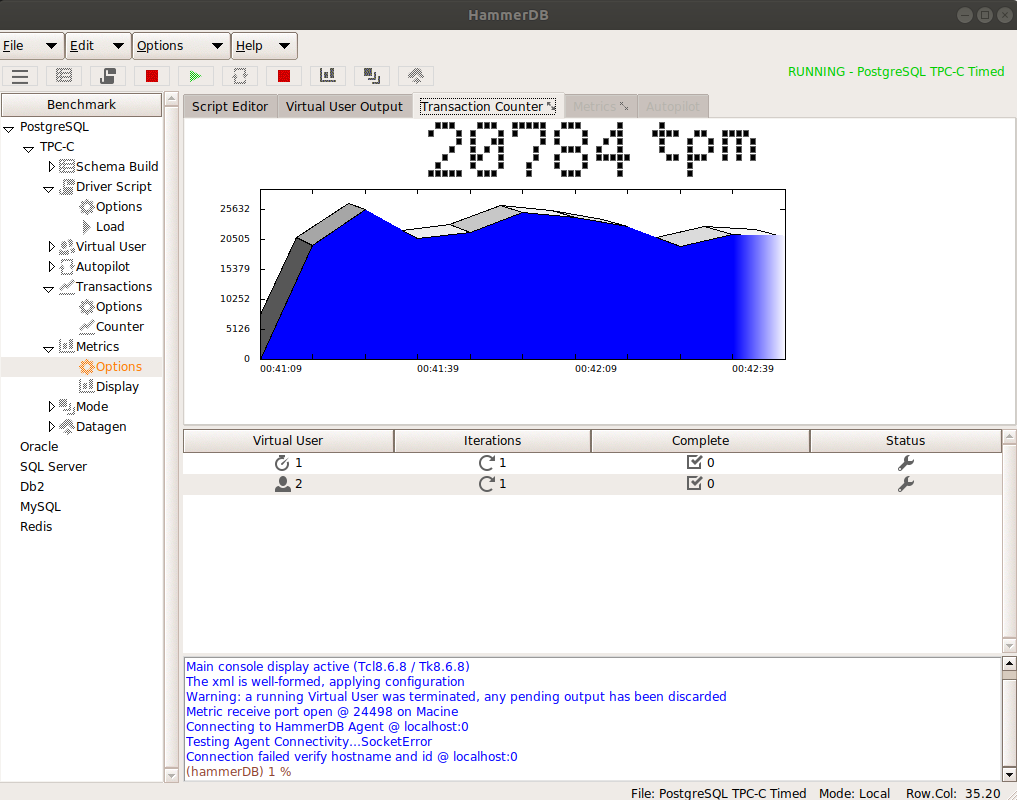
\includegraphics[width=0.6\columnwidth]{Chapters/images/hammerdb1.png}
        \caption{HammerDB GUI.}
    \label{fig:hamerdbgui}
    \end{figure}

Although HammerDB implements a workload based on the \gls{tpcc} specification, it does not implement a complete \gls{tpcc} benchmark specification. As a consequence,  the transaction results from HammerDB can not be compared  to the official \gls{tpcc} benchmarks. HammerDB workloads generate 2 statistics. \gls{tpm} is the transactional measurement of the specific database typically defined as the number of user commits plus the number of user rollbacks. \gls{tpm} values are database-specific and, thus, they cannot be compared among different \gls{dbms}. The \gls{nopm} value, on the other hand, is a performance metric independent of any particular database implementation and it is the recommended primary metric to use~\cite{hammerdb}.

%\discuss{Aqui tem vários screenshots do hammerDB que acho que fazia sentido teres um do género aqui:
%\url{https://www.hammerdb.com/about.html}}




HammerDB is being actively used by researchers to study the performance of DBMS: \citeauthor{elgrablyanalise} use HammerDB to compare open-source \gls{dbms} performance like Mysql, MariaDB and Postgres \cite{elgrablyanalise}. Another study that uses Hammerdb is \citeauthor{knoche2016combining}~(\citeyear{knoche2016combining}) work that uses HammerDB to test the impact of database lock contention in the \gls{tpcc} benchmark scenario~\cite{knoche2016combining}. In the context of green computing,  \citeauthor{koccak2018software}~(\citeyear{koccak2018software}) uses HammerDB with MySQL to define a dataset to use on his software energy consumption prediction~\cite{koccak2018software}. 

HammerDB is also being widely used by most leading database and technology companies, such as Oracle, IBM, Intel, Dell/EMC HPE, Huawei, Lenovo, and hundreds more~\cite{hammerdb}. It has been downloaded hundreds of thousands of times in more than 180 countries.




%\discuss{Dizer isto no capitulo seeguinte: aqui apenas descreves o hamerdb. No capitulos eguinte é que justificas o porquês de o usar}

%We decide to use HammerDB as it is a benchmark tool that can replicate the behavior of most cloud-based applications as a service, verify comprehensive performance and multiple metrics in a simple real-world environment on a virtual environment with virtual users~\cite{hammerdb}.

%Another reason we choose him was that HammerDB is used for automated software testing~\cite{hammerdb} so we can configure how many times the HammerDB will run and how many virtual users that he will use and for how long it will run, providing at the end of every execution the \gls{tpm} and the \gls{nopm}. With these numbers and the energy spent, we can have ample information to answer the RQ2, and with an adjustable number of users, it can assist in the RQ3.

